\documentclass[uplatex,dvipdfmx]{jsarticle}
\usepackage{geometry}
\pagestyle{empty}
\usepackage{tikz}
\usepackage{pgffor}
\usepackage{graphicx}
\usepackage[dvipdfmx]{animate}

\definecolor{CampbellBg}{HTML}{0C0C0C}
\definecolor{CampbellFg}{HTML}{CCCCCC}
\definecolor{CampbellBlack}{HTML}{0C0C0C}
\definecolor{CampbellBlue}{HTML}{0037DA}
\definecolor{CampbellCyan}{HTML}{3A96DD}
\definecolor{CampbellGreen}{HTML}{13A10E}
\definecolor{CampbellPurple}{HTML}{881798}
\definecolor{CampbellRed}{HTML}{C50F1F}
\definecolor{CampbellWhite}{HTML}{CCCCCC}
\definecolor{CampbellYellow}{HTML}{C19C00}
\definecolor{CampbellBrightBlack}{HTML}{767676}
\definecolor{CampbellBrightBlue}{HTML}{3B78FF}
\definecolor{CampbellBrightCyan}{HTML}{61D6D6}
\definecolor{CampbellBrightGreen}{HTML}{16C60C}
\definecolor{CampbellBrightPurple}{HTML}{B4009E}
\definecolor{CampbellBrightRed}{HTML}{E74856}
\definecolor{CampbellBrightWhite}{HTML}{F2F2F2}
\definecolor{CampbellBrightYellow}{HTML}{F9F1A5}

% vi: se ts=2 sw=2 et:


\newcommand{\docpaperwidth}{160mm}
\newcommand{\docpaperheight}{90mm}


\geometry{
  papersize={\docpaperwidth,\docpaperheight},
  margin=0cm,
  ignoreall=true
}
\setlength{\parindent}{0cm}

\usetikzlibrary{backgrounds}
\usetikzlibrary{calc}


% declare coordinates 
\newcommand{\coorddecl}{
 \coordinate (lbpos) at (0cm, 0cm);
 \coordinate (ltpos) at (0cm, \docpaperheight);
 \coordinate (rbpos) at (\docpaperwidth, 0cm);
 \coordinate (rtpos) at (\docpaperwidth, \docpaperheight);
}

% picgure bounding box
\newcommand{\bndbox}{
 (lbpos) rectangle (rtpos)
}

% picgure bounding box inset
\newcommand{\bndboxbi}{
 (0mm, 0mm) rectangle (\docpaperwidth, \docpaperheight - 8mm)
}

% internal img clip
\newcommand{\internalimg}{
  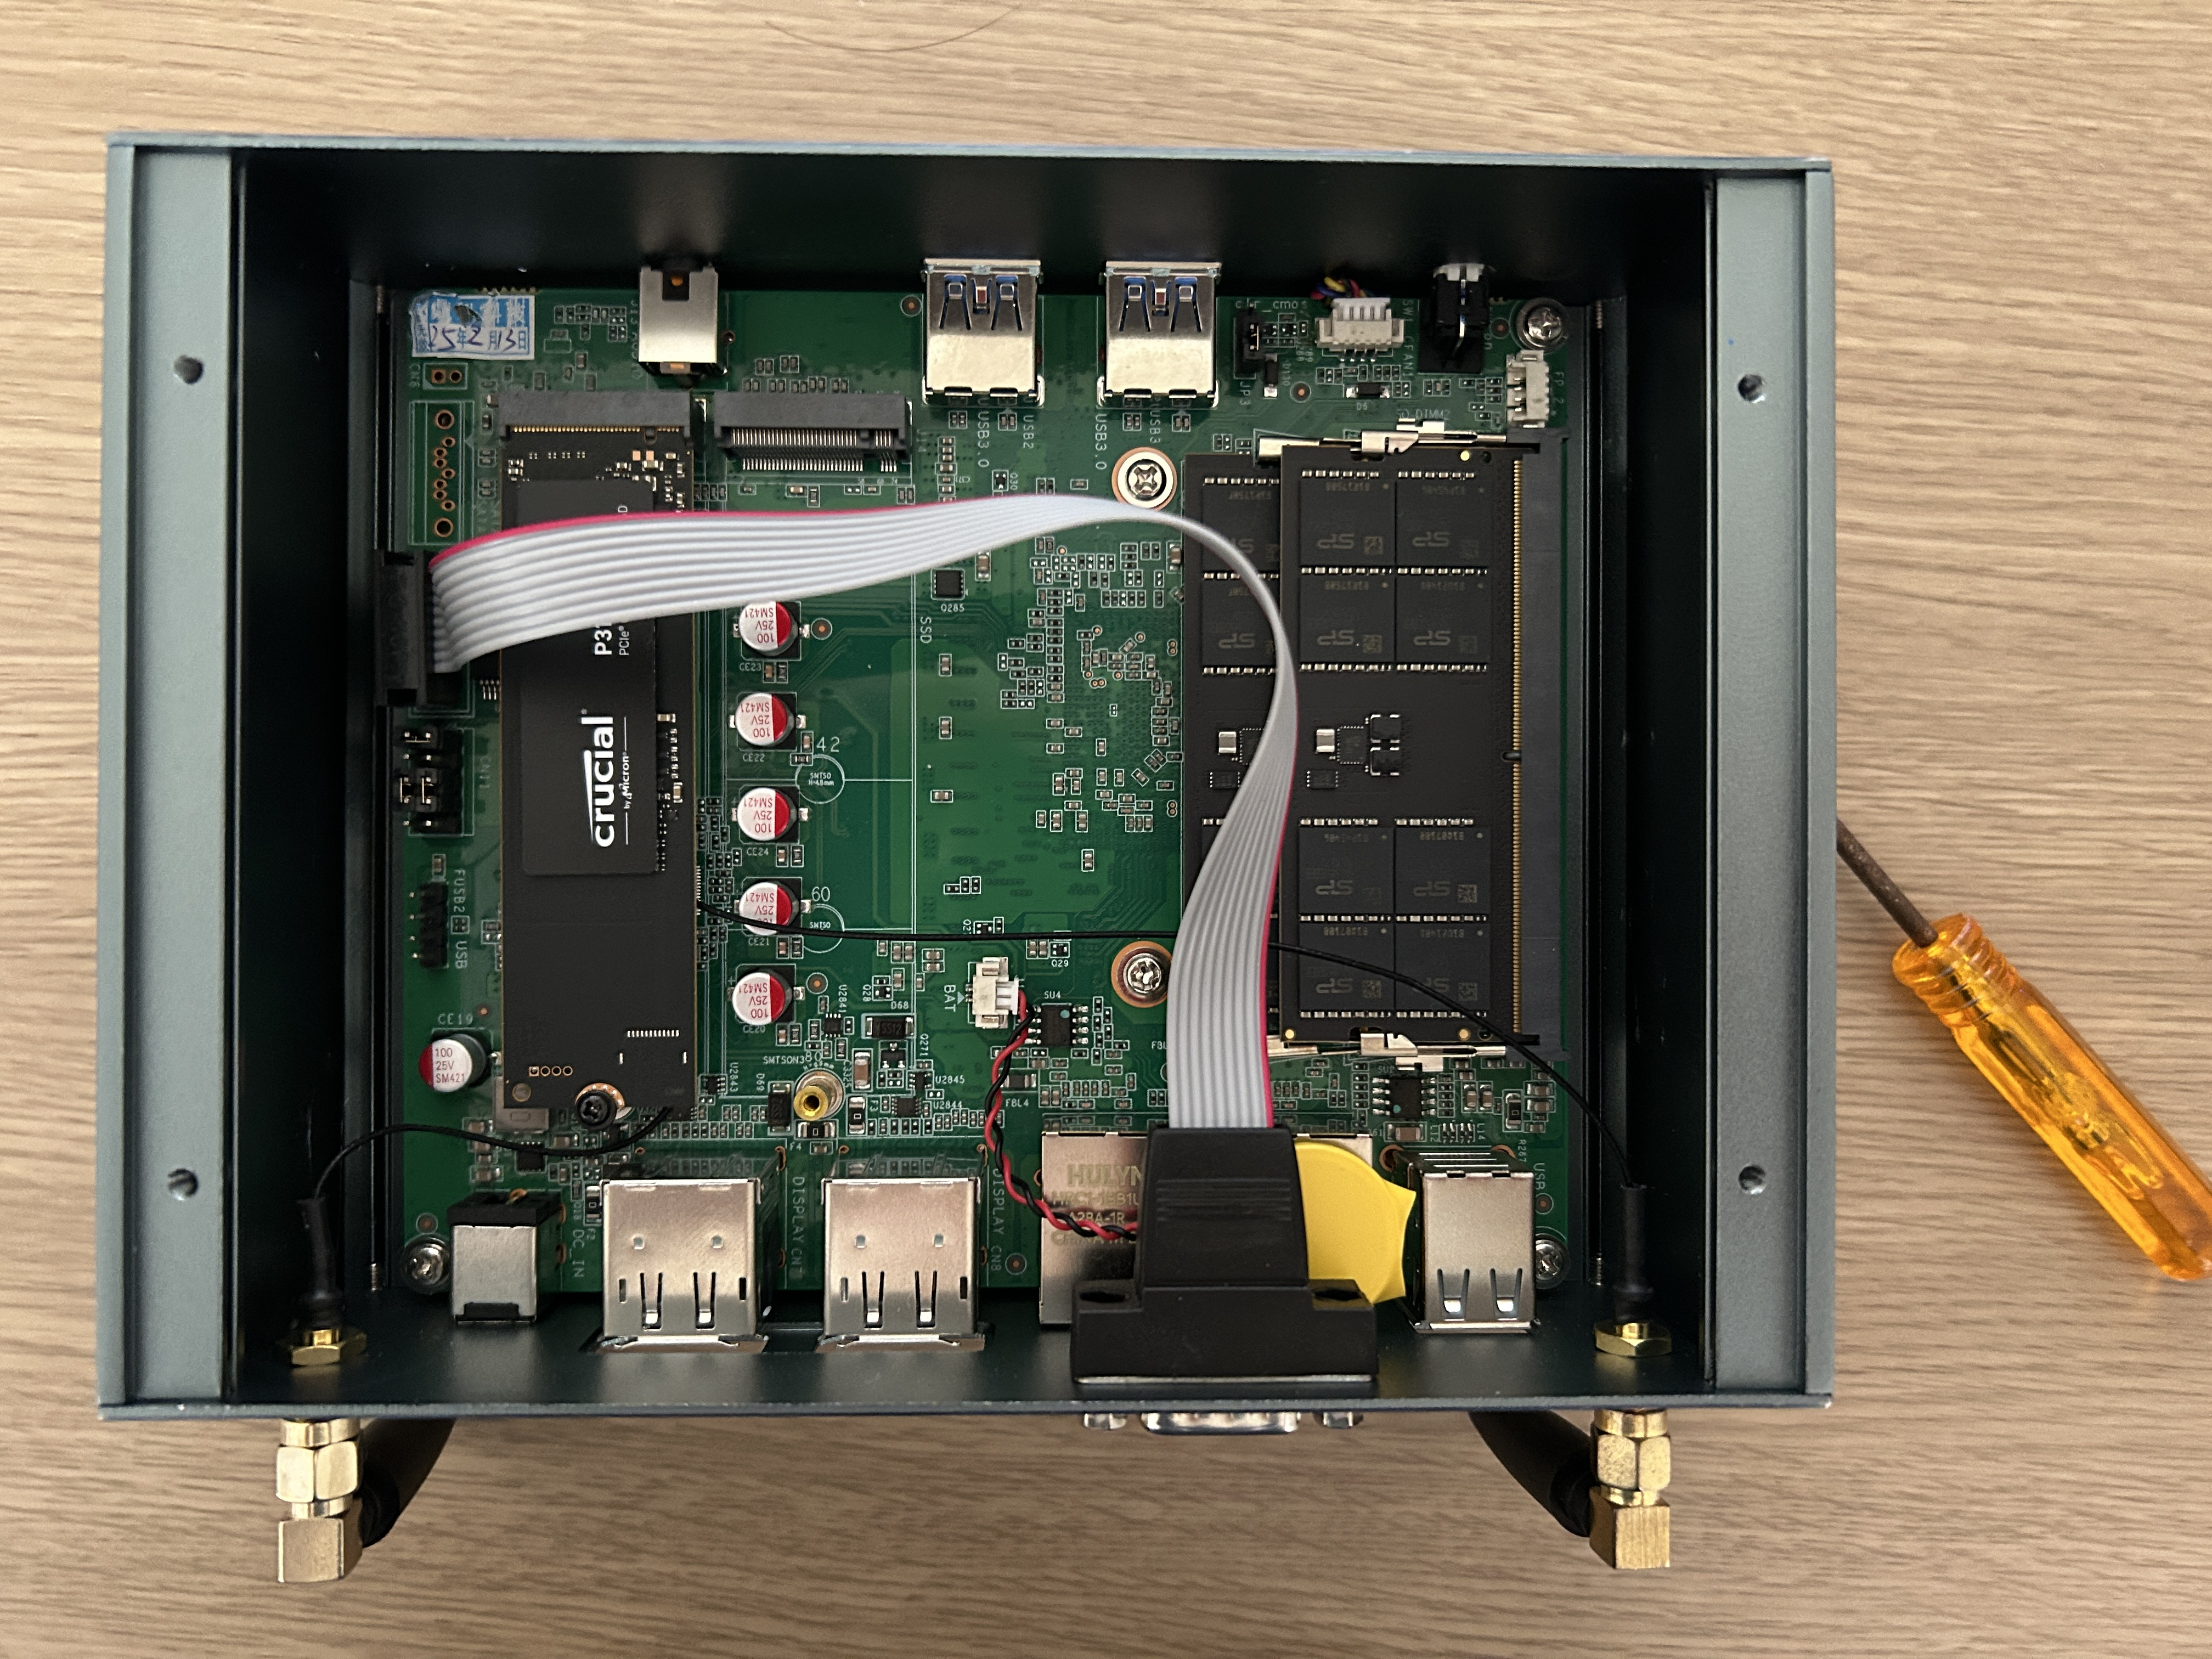
\includegraphics[
    clip,
    bb=0 0 3532 3024,
    height=4.5cm,
    page=1]{img/aiopcwa-internal-1.pdf}
}

\renewcommand{\familydefault}{\sfdefault}

% default color setting
\color{CampbellFg}
\pagecolor{CampbellBg}


\begin{document}
  \center
  %thumnail
  \begin{tikzpicture}
    \coorddecl
    \path [use as bounding box] \bndbox;
    \newcommand{\insarrow}{
       [xshift=38mm,yshift=40mm,rotate=90] (0mm,0mm) -- (5mm, 5mm)
        |- (18mm, 2.5mm) -- (18mm, -2.5mm)
        -| (5mm, -5mm) -- cycle}
    \node [anchor=center] at ($0.8*(ltpos) + 0.3*(rbpos)$){
     
\includegraphics[height=2.5cm,page=1]{img/archlinux-logo-dark-scalable.pdf}
    };
    \node [anchor=center] at ($0.8*(ltpos) + 0.65*(rbpos)$){
     \textsf{\LARGE{インストール}}
    };
    \begin{scope}
      \fill [color=CampbellBrightGreen] \insarrow;
    \end{scope}
    \draw [
      xshift=35.4mm,
      yshift=20mm,
      line width=0.25mm,
      color=CampbellBrightGreen]
     (0mm,0mm) [rounded corners=0.5mm] rectangle (5.2mm, 18mm);
    \begin{scope}[on background layer]
      \node [anchor=center] at ($0.3*(ltpos) + 0.3*(rbpos)$) {
        \internalimg
      };
    \end{scope}
  \end{tikzpicture}
  \newpage
  % head line page
  \begin{animateinline}[controls=true]{30}
    \multiframe{30}{isz=0+3} {
      \begin{tikzpicture}
      \coorddecl
      \path [use as bounding box] \bndboxbi;
      % arrow center x
      \newcommand{\arrowcx}{38mm}
      % arrow center y
      \newcommand{\arrowcy}{40mm}
      % arrow width half
      \newcommand{\arrowwh}{3mm}
      % arrow width quater
      \newcommand{\arrowwq}{1.5mm}
      % arrow length 
      \newcommand{\arrowl}{18mm}
      \newcommand{\insarrow}[2]{
         [xshift=\arrowcx+(#1pt),yshift=\arrowcy+(#2pt),rotate=90]
          (0mm,0mm) -- (\arrowwh, \arrowwh)
          |- (\arrowl, \arrowwq) -- (\arrowl, -\arrowwq)
          -| (\arrowwh, -\arrowwh) -- cycle}
      \newcommand{\instriangle}[4]{
         [xshift=(#3)+(#1),yshift=(#4)+(#2),rotate=90]
          (0mm,0mm) -- (\arrowwh, \arrowwh)
          -- (\arrowwh, -\arrowwh) -- cycle}
      \node [anchor=center] at ($0.75*(ltpos) + 0.3*(rbpos)$){
         
\includegraphics[height=1.8cm,page=1]
           {img/archlinux-logo-dark-scalable.pdf}
      };

      \begin{scope}[on background layer]
        \clip 
          (\docpaperwidth * 0.3 - \isz mm * 0.3532, 
           \docpaperheight * 0.3 - \isz mm * 0.3024)
          rectangle
          (\docpaperwidth * 0.3 + \isz mm * 0.3532, 
           \docpaperheight * 0.3 + \isz mm * 0.3024);
        \node [anchor=center] at ($0.3*(ltpos) + 0.3*(rbpos)$) {
          \internalimg
        };
      \end{scope}
      \end{tikzpicture}
    }
    \newframe
    \multiframe{30}{no=0+0.03333}{
      \begin{tikzpicture}
        \coorddecl
        \path [use as bounding box] \bndboxbi;
        % arrow center x
        \newcommand{\arrowcx}{38mm}
        % arrow center y
        \newcommand{\arrowcy}{40mm}
        % arrow width half
        \newcommand{\arrowwh}{3mm}
        % arrow width quater
        \newcommand{\arrowwq}{1.5mm}
        % arrow length 
        \newcommand{\arrowl}{18mm}
        \newcommand{\insarrow}[2]{
           [xshift=\arrowcx+(#1pt),yshift=\arrowcy+(#2pt),rotate=90]
            (0mm,0mm) -- (\arrowwh, \arrowwh)
            |- (\arrowl, \arrowwq) -- (\arrowl, -\arrowwq)
            -| (\arrowwh, -\arrowwh) -- cycle}
        \newcommand{\instriangle}[4]{
           [xshift=(#3)+(#1),yshift=(#4)+(#2),rotate=90]
            (0mm,0mm) -- (\arrowwh, \arrowwh)
            -- (\arrowwh, -\arrowwh) -- cycle}
        \node [anchor=center] at ($0.75*(ltpos) + 0.3*(rbpos)$){
           
\includegraphics[height=1.8cm,page=1]
             {img/archlinux-logo-dark-scalable.pdf}
        };
        \begin{scope}[on background layer]
          \node [anchor=center] at ($0.3*(ltpos) + 0.3*(rbpos)$) {
            \internalimg
          };
        \end{scope}
        \draw [
          xshift=35.4mm,
          yshift=20mm,
          line width=0.25mm,
          color=CampbellBrightGreen,
          opacity=\no]
         (0mm,0mm) [rounded corners=0.5mm] rectangle (5.2mm, 18mm);
      \end{tikzpicture}
    }
    \newframe 
    \multiframe{30}{no=0+0.03333}{
      \begin{tikzpicture}
        \coorddecl
        \path [use as bounding box] \bndboxbi;
        % arrow center x
        \newcommand{\arrowcx}{38mm}
        % arrow center y
        \newcommand{\arrowcy}{40mm}
        % arrow width half
        \newcommand{\arrowwh}{3mm}
        % arrow width quater
        \newcommand{\arrowwq}{1.5mm}
        % arrow length 
        \newcommand{\arrowl}{18mm}
        \newcommand{\insarrow}[2]{
           [xshift=\arrowcx+(#1pt),yshift=\arrowcy+(#2pt),rotate=90]
            (0mm,0mm) -- (\arrowwh, \arrowwh)
            |- (\arrowl, \arrowwq) -- (\arrowl, -\arrowwq)
            -| (\arrowwh, -\arrowwh) -- cycle}
        \newcommand{\instriangle}[4]{
           [xshift=(#3)+(#1),yshift=(#4)+(#2),rotate=90]
            (0mm,0mm) -- (\arrowwh, \arrowwh)
            -- (\arrowwh, -\arrowwh) -- cycle}
        \node [anchor=center] at ($0.75*(ltpos) + 0.3*(rbpos)$){
           
\includegraphics[height=1.8cm,page=1]
             {img/archlinux-logo-dark-scalable.pdf}
        };
        \begin{scope}[on background layer]
          \node [anchor=center] at ($0.3*(ltpos) + 0.3*(rbpos)$) {
            \internalimg
          };
        \end{scope}
        \draw [
          xshift=35.4mm,
          yshift=20mm,
          line width=0.25mm,
          color=CampbellBrightGreen]
         (0mm,0mm) [rounded corners=0.5mm] rectangle (5.2mm, 18mm);
        \begin{scope}
          \clip (\arrowcx - \arrowwh - 1mm, \arrowcy - 1mm)
            rectangle (\arrowcx + \arrowwh + 1mm, \arrowcy + 4 * 5mm);
          \foreach \yd in {0,5,...,25}
            {
              \fill [color=CampbellBrightGreen, opacity=\no]
                \instriangle{0}{0}{\arrowcx}{\arrowcy + \yd mm};
            }
        \end{scope}
      \end{tikzpicture}
    }
  \end{animateinline}
  \newpage
  \begin{animateinline}[controls=true,loop]{30}
    \multiframe{20}{ny=0+0.25}{
      \begin{tikzpicture}
      \coorddecl
      \path [use as bounding box] \bndboxbi;
      % arrow center x
      \newcommand{\arrowcx}{38mm}
      % arrow center y
      \newcommand{\arrowcy}{40mm}
      % arrow width half
      \newcommand{\arrowwh}{3mm}
      % arrow width quater
      \newcommand{\arrowwq}{1.5mm}
      % arrow length 
      \newcommand{\arrowl}{18mm}
      \newcommand{\insarrow}[2]{
         [xshift=\arrowcx+(#1pt),yshift=\arrowcy+(#2pt),rotate=90]
          (0mm,0mm) -- (\arrowwh, \arrowwh)
          |- (\arrowl, \arrowwq) -- (\arrowl, -\arrowwq)
          -| (\arrowwh, -\arrowwh) -- cycle}
      \newcommand{\instriangle}[4]{
         [xshift=(#3)+(#1),yshift=(#4)+(#2),rotate=90]
          (0mm,0mm) -- (\arrowwh, \arrowwh)
          -- (\arrowwh, -\arrowwh) -- cycle}
      \node [anchor=center] at ($0.75*(ltpos) + 0.3*(rbpos)$){
         
\includegraphics[height=1.8cm,page=1]
           {img/archlinux-logo-dark-scalable.pdf}
      };
      \begin{scope}[on background layer]
        \node [anchor=center] at ($0.3*(ltpos) + 0.3*(rbpos)$) {
          \internalimg
        };
      \end{scope}
      \draw [
        xshift=35.4mm,
        yshift=20mm,
        line width=0.25mm,
        color=CampbellBrightGreen]
       (0mm,0mm) [rounded corners=0.5mm] rectangle (5.2mm, 18mm);

      \begin{scope}
        \clip (\arrowcx - \arrowwh - 1mm, \arrowcy - 1mm)
          rectangle (\arrowcx + \arrowwh + 1mm, \arrowcy + 4 * 5mm);
        \foreach \yd in {0,5,...,25}
          {
            \fill [color=CampbellBrightGreen]
              \instriangle{0}{-\ny mm}{\arrowcx}{\arrowcy + \yd mm};
          }
      \end{scope}
   \end{tikzpicture}
  }
  \end{animateinline}
\end{document}

% vi: se ts=1 sw=2 et:
